% SyncBox manual - Command Interface
% Written by Christopher Thomas.
%
% Copyright (c) 2021 by Vanderbilt University. This work is released under
% the Creative Commons Attribution-ShareAlike 4.0 International License.

\chapter{Command Interface}
\label{sect-commands}

The {\projectname} is connected to the host computer via a USB serial link at 
115200 baud. The host issues commands, and the {\projectname} reports events 
that occur.

The {\projectname} issues timing pulses at regular intervals; issues reward 
pulses as one-off events; writes parallel event code data to the ephys I/O
port; and reports analog input from the joystick and light sensors at regular 
intervals.

In addition to analog light sensor values, the {\projectname} also reports
whether each sensor is above- or below-threshold. Light sensor thresholds
are calibrated by measuring sensor values during a time window, taking the 
average of these measured values, and then saving the average as the new 
threshold (overwriting the old threshold). 
``Free-running'' calibration does this repeatedly (starting a new window 
when the old window ends).

A list of available commands is shown in Figure \ref{fig-commands}. A timing
diagram of user-commanded output events is shown in Figure \ref{fig-timing}.
A diagram illustrating light sensor filtering is shown in Figure
\ref{fig-filtering}.

\begin{figure}[p]
\verbatiminput{captures/capture-help.txt}
\caption{Command summary.}\label{fig-commands}
\end{figure}

\begin{figure}[p]
\begin{center}
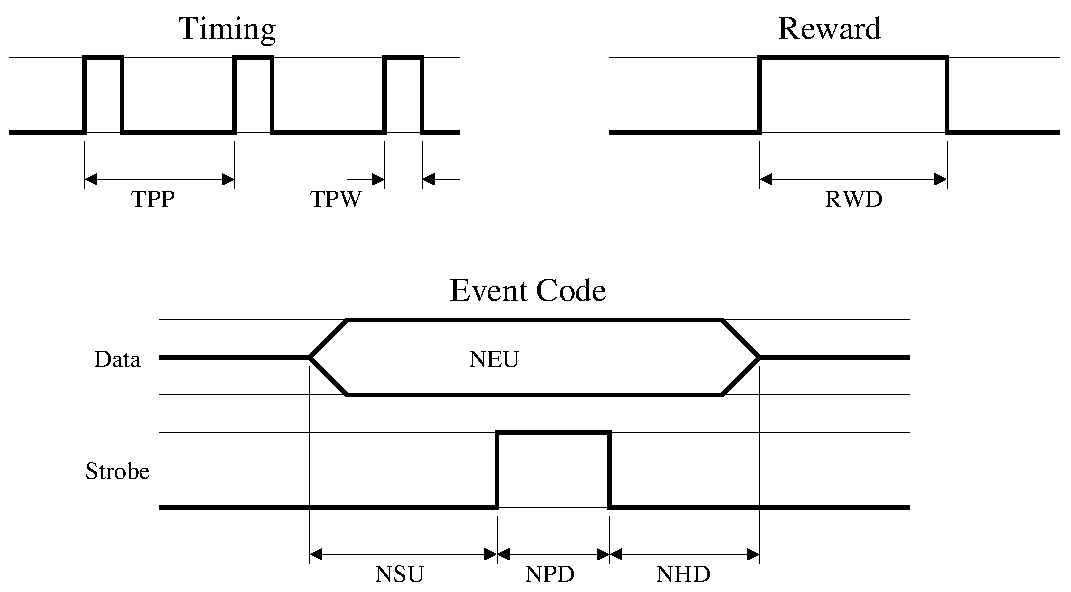
\includegraphics[height=3in]{figs/timing.pdf}
\end{center}
\caption{Output signal timing diagram.}\label{fig-timing}
\end{figure}

\begin{figure}[p]
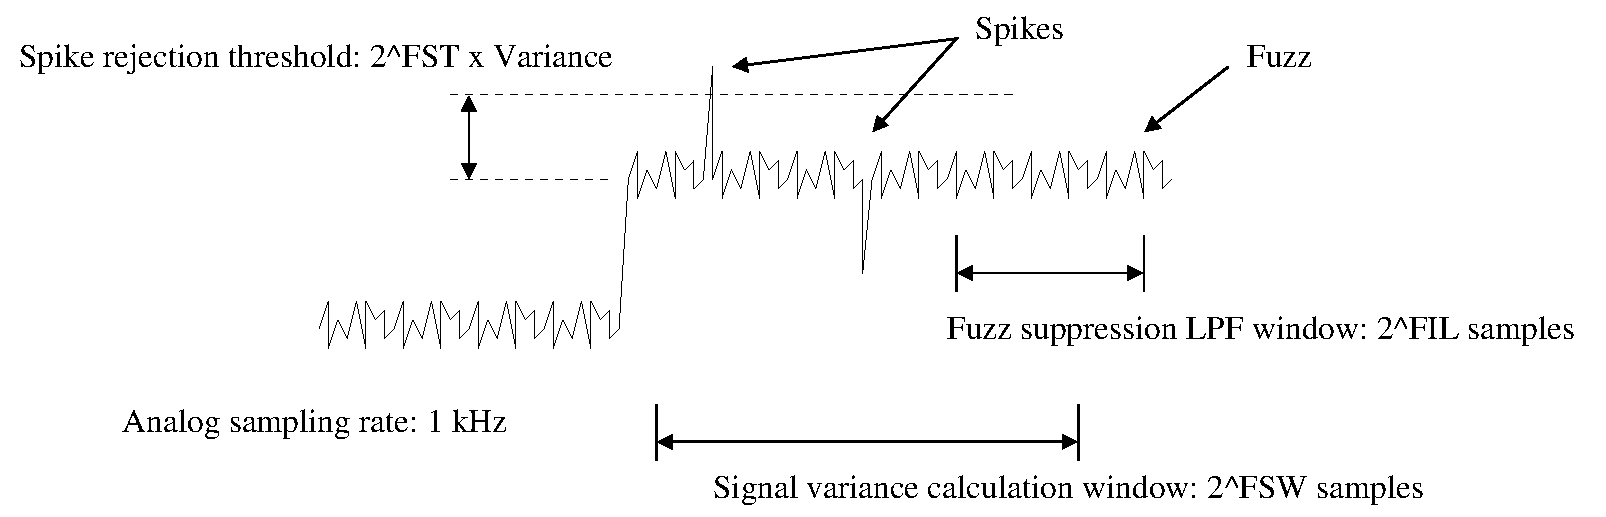
\includegraphics[width=0.95\textwidth]{figs/swfilter.pdf}
\caption{Light sensor filtering.}
\label{fig-filtering}
\end{figure}

Sample output (including echoed commands) is shown in Figure 
\ref{fig-output}. Format details for verbose, terse, and packed log entries
are given in Figure \ref{fig-formats}. Typical configuration/status
information is shown in Figure \ref{fig-status}.

There are several important things to note about interactions with the 
{\projectname}:

\begin{itemize}
\item The command parser does \textbf{not} recognize backspaces.

\item \textbf{All times}, whether they're timestamps or duration 
arguments, are given in \textbf{``clock ticks'', not milliseconds}. By 
default, clock ticks are 0.1~ms in length. One second is 10000 ticks.

Milliseconds would not have been sufficiently precise, and microseconds 
would have overflowed a 32-bit counter in slightly more than one hour.

Bear in mind that the maximum argument value is 65535 (a duration or 
interval of about 6.5 seconds).

% FIXME - Force a page break.
\clearpage
\item Number values entered by the user are given in \textbf{decimal}, but 
number values reported from the {\projectname} are in \textbf{hexadecimal} 
(with the exception of status information).

Processing user information in decimal made the command parser simpler 
(and makes life easier for manually entering data). Reporting information 
in hexadecimal makes output more compact (important for high data rate 
output), and avoids time-consuming data conversion (converting to 
hexadecimal does not require divisions, only bit-shifts; converting to 
decimal does require divisions). The data rate is high enough that this 
matters.
\end{itemize}

The data reporting rate is limited by the serial connection. If events 
occur too fast to report (or if full-rate analog debug reporting exceeds the
serial connection's ability to report), reports will be dropped. Events 
themselves will still occur.

At 115200 baud, the maximum reporting rate without packet loss is 150~Hz
with verbose logging, 200~Hz with terse logging, and 300~Hz with packed
hex logging.

\begin{figure}[p]
\verbatiminput{captures/capture-messages.txt}
\caption{Sample {\projectname} output.}\label{fig-output}
\end{figure}

\begin{figure}[p]
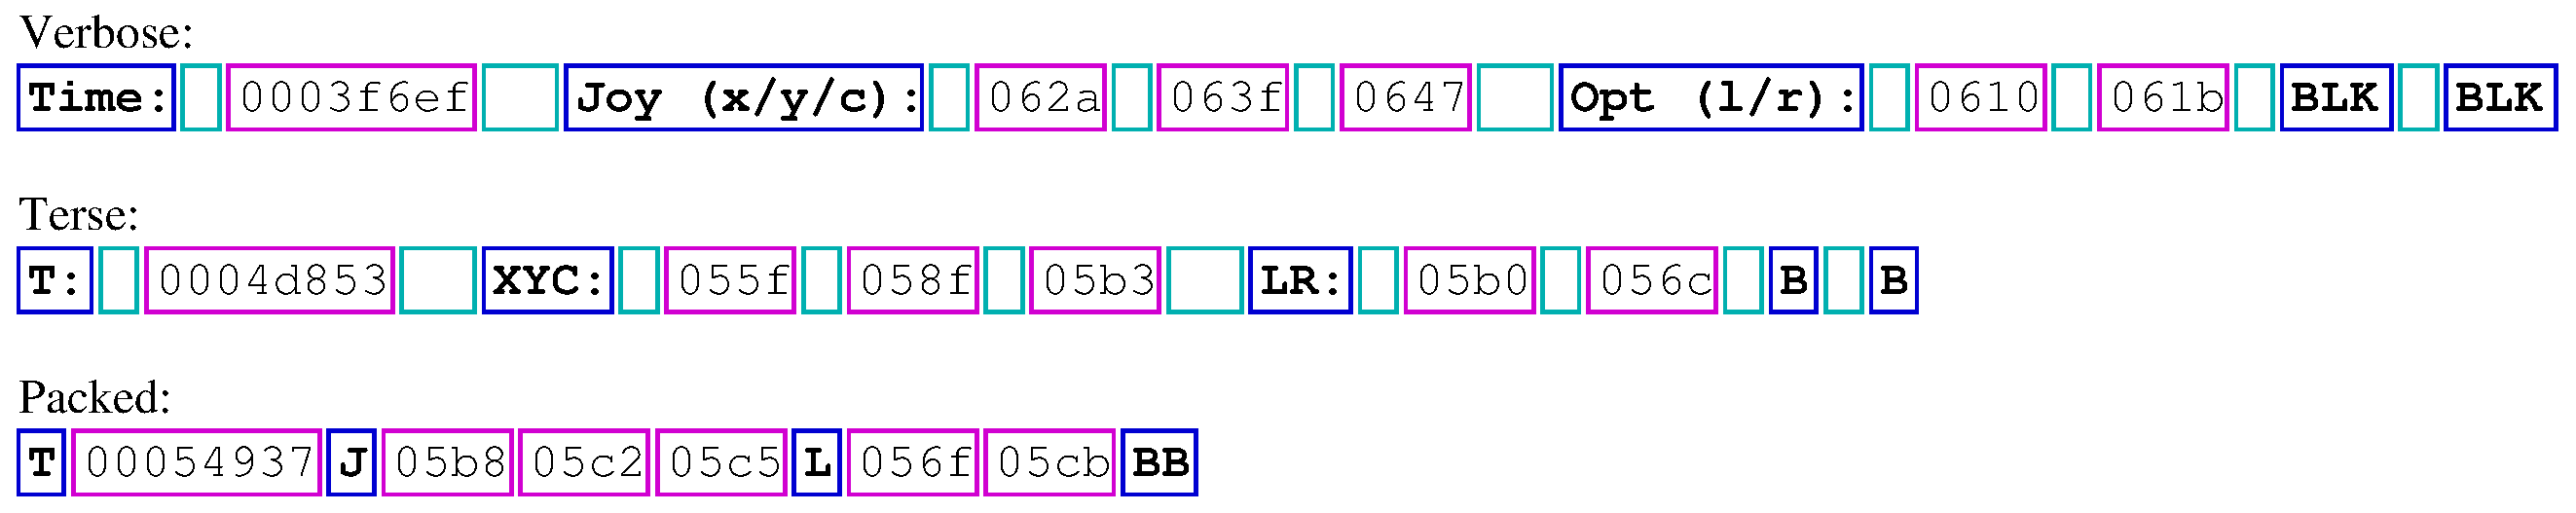
\includegraphics[width=0.95\textwidth]{figs/formats.pdf}
\caption{Log entry format details.}
\label{fig-formats}
\end{figure}

\begin{figure}[p]
\verbatiminput{captures/capture-status.txt}
\caption{{\projectname} identification string and status report.}
\label{fig-status}
\end{figure}

%
% This is the end of the file.
